\documentclass{article}
\usepackage[utf8]{inputenc}
\usepackage{graphicx}
\usepackage[left=2cm, right=2cm]{geometry}
\setlength{\parindent}{0pt}

\usepackage{color}
\usepackage{float}
\usepackage{amsmath}
\usepackage{amssymb}
\usepackage{multirow}
%\usepackage[style=numeric, backend=biber]{biblatex} 


\usepackage[style=numeric,doi=false,isbn=false,url=false]{biblatex}
\addbibresource{zotero_references.bib}

%\usepackage[numbers]{natbib}   
%\bibliographystyle{FG_AK_English_Number}
%\bibliographystyle{apa}

\title{Master Thesis Exposé}
\author{William Rodewald}
\date{\today}

\newcommand{\comment}[1]{{\color{red}{[#1]}}}

\newcommand\pro{\item[$+$]}
\newcommand\con{\item[$-$]}

\usepackage{array}
\newcolumntype{?}{!{\vrule width 1pt}}

\begin{document}

\maketitle

\tableofcontents

\newpage
 
\section{Abstract}
\comment{ The abstract summarizes the exposés content. }\\

\section{Introduction and Motivation}
\label{sec:Intro}
\comment{This sections introduces the motivation and research goals for this thesis.}\\

% While Vocaloid receives success in Asia not only as a software for singing voice synthesis but also as the umbrella term for virtual avatars such as Hatsune Miku \cite{le_examining_2015}, both the software and the avatars are relatively unknown in America and Europe.

In today's music production, virtual acoustic instruments are a viable alternative to acoustic instruments. Virtual violins, pianos and guitars are a common appearance in music studios. Virtual singers however are still a relative rarity in the world of music production. \comment{citation needed} This might be explained by the complexity of the human voice compared to most acoustic instruments. Not only does the human voice introduce a semantic factor into music, an aspect not found in other acoustic instruments. We are also trained to recognize the human voice and distinguish it from other voices from an early age.

The rarity of natural voice synthesizers in the music software industry however does not stem from a lack of research in the field of singing voice synthesis. Early methods for voice synthesis such as the source-filter model \cite{fant_acoustic_1960}, dating back to 1960, have now been succeeded by end-to-end approaches such as WaveNet \cite{oord_wavenet:_2016} and vocoder based neural network approaches \cite{chandna_wgansing:_2019}\cite{blaauw_neural_2017}. These state of the art methods provide fully phonetic models that can be used to synthesize sung text phrases with the control over both the text (phonation) and musical score (pitch, expression). However, they do so for a relatively high computational cost that might not fulfil the requirements of some application cases. 

\begin{figure}[H]
    \centering
    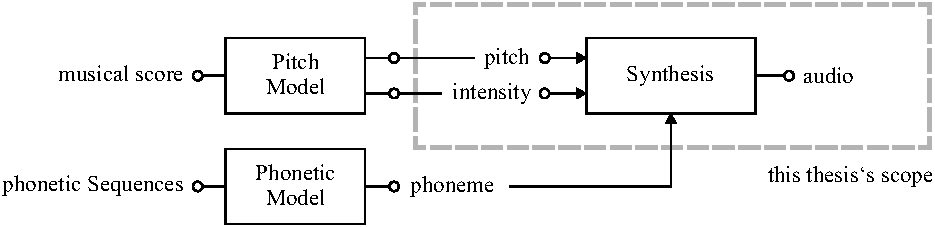
\includegraphics{Graphics/004_thesis_scope.pdf}
    \caption{A text-to-speech singing voice synthesis architecture might consist of a phonetic model, a pitch estimation model and a synthesis model. This thesis scope is limited on the latter.}
    \label{fig:thesis_architecture_scope}
\end{figure}

One possible architecture for a singing voice synthesis model is shown in figure \ref{fig:thesis_architecture_scope}. While the two control parameters pitch and intensity can be controlled directly, they can also be generated from a music score. Phonetic singing voice synthesis methods also include some form of phonetic model, either as a separate component or by conditioning networks using phonemes.\\
In this thesis we want to focus on highly efficient singing voice synthesis, incorporating advances of the past years into classic digital signal processing. To achieve this, this thesis's scope is narrowed down to the synthesis of sung vowels. We therefore do not include a phonetic model or discuss the topic of pitch modelling.
Furthermore, we aim for a multi-singer model, that not only allows voice synthesis using different voice timbre qualities but also morphing between those qualities to create new virtual singers. For analysis, the VocalSet dataset \cite{wilkins_vocalset:_2018} is used to extract pitch and intensity trajectories as well as voice timbre qualities for different virtual singers. This thesis's research questions are as follows:

\begin{itemize}
    \item What methods provide exceptional computational efficiency while still capturing singers voice timbre qualities?
    \item How can we morph efficiently between virtual voices without loosing naturalness?
    \item What validation methods prove suitable for evaluating the naturalness of both synthesized and morphed, synthesized voices.
\end{itemize}

Answering these questions will help us understand important aspects of singing voice synthesis. What might a minimal model for a virtual voice look like that still manages to capture the singers voice qualities? What aspects of a voice are critical for its perception as natural and not synthetic. Application cases for the proposed method can be found in the music software industry. Some scenarios are the implementation of digital choirs or the synthesis of backing or harmonization vocals.\\

With singing voice synthesis being a highly researched topic, the limited scope considered in  this thesis is supposed to help in two ways. Firstly, we aim to differentiate this thesis from existing research. Secondly the limited scope is supposed to reduce the expected workload to a manageable amount, considering the time frame of the thesis of six months and the authors lack of prior knowledge on the topic of singing voice synthesis. \comment{Not sure if this "meta" block is necessary.}


\section{Current State of Research}

\subsection{Voice Production System}

\begin{figure} [H]
    \centering
    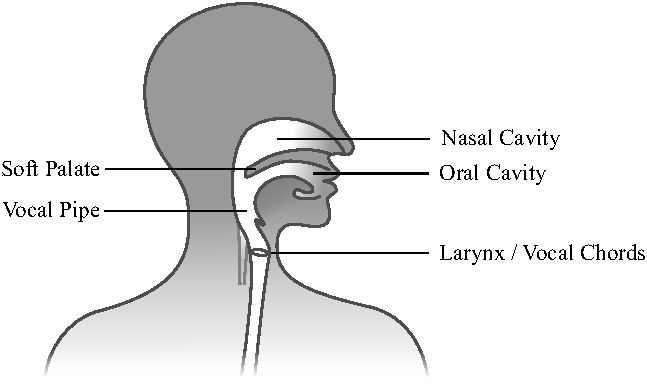
\includegraphics{Graphics/002_VoiceProduction_Physiology.pdf}
    \caption{The human physiology of the organs responsible for the voice production.}
    \label{fig:physiology}
\end{figure}

Early models of the human voice production system were already proposed back in the 1940s \cite{chiba_vowel_1942}. Later on, the source-filter model was widely adopted as a simplified model for the voice production. It was originally proposed in 1960 in \cite{fant_acoustic_1960} but the concept was already explored in experiments with the first vocoder in \cite{dudley_vocoder_1939}, \cite{dudley_remaking_1939}. The source-filter model separates the human voice production in the source and the filter. The source is usually represented by the vocal chords as the organ that initially creates a vibrating air volume, usually referred to as the glottal flow. The filter is represented by vocal tract consisting of the vocal pipe, oral and nasal cavity. The vocal tract filters the glottal flow, creating resonances or formants in the spectrum. \\
There are many ways for a singer to shape the sound. Singers can sing in different registers or phonation modes\cite{sundberg_science_1987} by adjusting the shape of the vocal chords \cite{salomao_what_2009}. The larynx, or voice box, that contains the voice chords, can be moved slightly up and down by singers, shortening or lengthening the vocal tract to alter the filters spectral envelope \cite{sundberg_raised_1976}. By closing the soft palate, singers can decouple the nasal cavity from the remaining vocal tract to again alter the spectral envelope of the filter \cite{elie_characterisation_2009}. Additionally, The singer has control over the filter spectral envelope by shaping the vocal tract, i.e. by moving the tongue or the lips.

\subsection{Voice Qualities}

In \cite{sundberg_perceptual_1994}, the author classifies voice qualities into timbre, pitch and loudness with timbre qualities being differentiated again in vowel and voice qualities. 
Timbre qualities are mostly controlled by the shape and length vocal tract, and determine the perceived vowel (1st and 2nd formant) and the voice timbre (higher formants). The perceived loudness is not only affected by the overall amplitude but also by the ratio between higher and lower overtone. Temporal variations in pitch, loudness, timbre and phonation are referred to as expression. 

\subsection{Singing Voice Synthesis}

\begin{figure}[H]
    \centering
    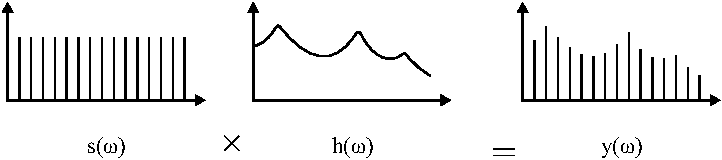
\includegraphics{Graphics/003_SourceFilter_1960.pdf}
    \caption{The source-filter model as proposed in \cite{fant_acoustic_1960}.}
    \label{fig:source_filter}
\end{figure}

Based on early models of the voice production system, some of the first singing voice synthesis methods were source-filter model as described in \cite{fant_acoustic_1960}. The original paper proposes a flat harmonic glottal flow model such as an impulse train as the source $s(\omega)$. The filter $h(\omega)$ could be implemented as an all-pole system that would shaped the vowels formants of the output signal $y(\omega)$ as shown in figure \ref{fig:source_filter}. This model only requires estimation of pitch and the spectral envelope $h(\omega)$. For the purpose of spectral envelope estimation, many methods have been suggested. Linear prediction (LP) was proposed early on \cite{makhoul_linear_1975} with a revised pitch synchronous model (PS LP) proposed in \cite{guerchi_pitch-synchronous_2000}. True Envelope (TE), originally proposed in 1979 \cite{imai_spectral_1979} was rediscovered in 2005 \cite{roebel_efficient_2005}\cite{villavicencio_improving_2006} as one alternative method for spectral envelope estimation. TE iteratively smears the spectrum prior to linear prediction by filtering in the quefreuncy domain to prevent the spectral envelope from overfitting harmonic peaks, an issue commonly seen in LP especially with high pitched signals. More recent methods for spectral envelope estimation include CheapTrick \cite{morise_cheaptrick_2015} or multi frame analysis methods\cite{degottex_simple_2016}.\\

Early on, it was noted that a flat harmonic spectrum is a poor approximation for the glottal flow as the original source-filter model proposed. For that reason, alternative models for the glottal flow, such as the 4-parameter LF model \cite{fant_four-parameter_1985} and the revised 1-parameter LF-$R_d$ model \cite{fant_lf-model_1995} were presented. Source-filter models that see the use of non-flat harmonic signals as the source signal or extend the source-filter model otherwise are usually referred to extended source-filter model. With the introduction of parametric glottal flow models however, the task of separating source and filter is non-trivial. Many methods for source-filter separation were proposed \cite{jinachitra_joint_2005}\cite{degottex_glottal_2010}\cite{perrotin_spectral_2019}. Joint estimation methods provide the means to estimate both source and filter simultaneously. In \cite{loweimi_source-filter_2015}, separation is achieved by analysing trends and fluctuations in the phase domain. Other methods rely on optimization algorithms such as differential evolution \cite{schleusing_joint_2013}.\\

For synthesis of full spoken or sung phrases, concatenative systems \cite{schwarz_concatenative_2006} were proposed. 

\subsection{Machine Learning in Singign Voice Synthesis}

More recently, machine learning methods for end-to-end singing voice synthesis systems were proposed. These include WaveNet \cite{oord_wavenet:_2016}, an autorregressive neural network that was proposed for the use of text-to-speech or singing voice synthesis. A WaveNet is trained to predict the next sample of an audio sequence and, during generation, uses the predicted sample as it's own input. In \cite{blaauw_neural_2017}, a WaveNet structure was used in conjunction with the WORLD vocoder\cite{morise_world:_2016}. The vocoder extracts spectral envelope coefficients, pitch and an aperiodicity measure from audio and uses the same to recreate the signal. The proposed model uses a modified WaveNet structure to predict the vocoder parameters instead of raw audio. This takes the burden of separating pitch and timbre from the network. As a compromise, any prediction errors in the vocoder analysis or synthesis can't propagate back through the network, resulting in a worse performance than end-to-end approaches \cite{engel_ddsp:_2020}. A similar approach, using Generative Adversarial Networks (GAN) instead of WaveNet for vocoder parameter prediction, is presented in \cite{chandna_wgansing:_2019}. Other approaches include WaveRNN \cite{kalchbrenner_efficient_2018}, based on recurrent neural networks (RNN) and \cite{nakamura_singing_2019}, based on Convolutional Neural Networks.\\

Very recently, differentiable digital signal processing (DDSP) was proposed as a method for combining classical digital signal processing with deep neural networks \cite{engel_ddsp:_2020}. The authors suggested the use of differentiable DSP components such as additive synthesis or FIR filter that could be included in neural networks. The proposed autoencoder architecture uses a decoder to extract pitch, loudness and other latent space control variables from an audio input. The decoder then uses these control variables to predict the coefficients for the DSP components to synthesize the original. Since the dsp components are differentiable, the full architecture can propagate back errors in the synthesized signal and thus can be trained as one network. 


\subsection{Morphing Singers}

For source-filter models, it was suggested early on that the line spectral frequency (LSF)\cite{itakura_line_1975} representation of all-pole filters shows desirable interpolation characteristics. In \cite{roddy_method_2014} the use of LSF was proposed as a method of morphing between spectral envelopes. 


\section{Methods}

\subsection{Dataset}

This thesis uses the VocalSet dataset \cite{wilkins_vocalset:_2018}. The dataset consists of sung vowel excerpts from 20 singers (9 female, 11 male). For each singer, five vowels are sung in different arrangements (single notes, arpeggios and scales) and different singing techniques (vibrato, straight, breathy,...). 

\subsection{Singing Voice Synthesis}

\begin{figure}[H]
    \centering
    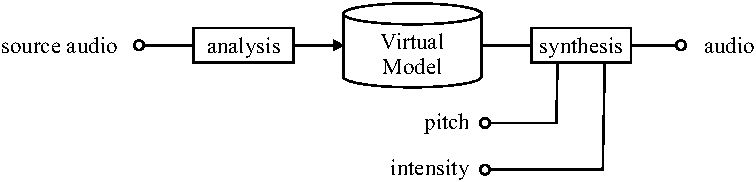
\includegraphics{Graphics/005_method_singer_model.pdf}
    \caption{A singer model is trained from source audio material. The model is used with pitch and control parameters to generate new sung vowels.}
    \label{fig:singer_model}
\end{figure}

In this thesis, we aim to propose a singing voice synthesis method for the synthesis of sung vowels. For this purpose, we train virtual singer model using target source samples from the VocalSet. During synthesis, these models can be used with control parameters pitch and intensity to synthesize new excerpts. Furthermore, singer models can be morphed, either during analysis or synthesis, to blend between voice timbre qualities. An overview is shown in figure \ref{fig:singer_model}.\\

After reviewing the current sate of research, three types of approaches were deemed suitable. These include end-to-end \textbf{audio prediction} approaches like WaveNet \cite{oord_wavenet:_2016}, spectral envelope / \textbf{vocoder prediction} approaches like WGANSing \cite{chandna_wgansing:_2019} and \textbf{extended source-filter} models extracted from source audio \cite{schleusing_joint_2013}. These three  approaches differ in abstraction, required domain knowledge and computational efficiency. Audio prediction methods achieve very good results with low required domain knowledge at the cost of accuracy while extended source filter models require a high level of domain knowledge and perform worse then state at the art methods for the benefit of computational efficiency. A comparison is shown in figure \ref{fig:method_comparison}. In the following sections, all three approaches are briefly introduced. 

\begin{figure}[H]
    \centering
    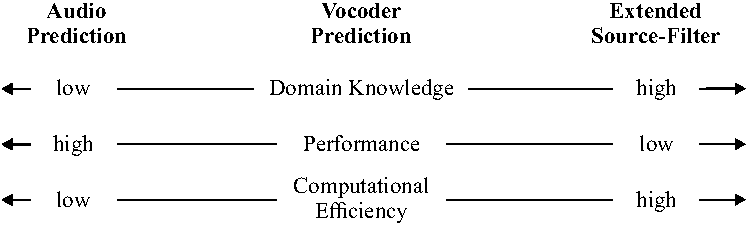
\includegraphics{Graphics/006_method_compairson.pdf}
    \caption{Compared to extended source-filter models, audio predictor approaches trade low required domain knowledge and a better accuracy with a low computational efficiency.}
    \label{fig:method_comparison}
\end{figure}

\subsubsection*{End-to-End Audio Predictor Methods}

\begin{figure}[H]
    \centering
    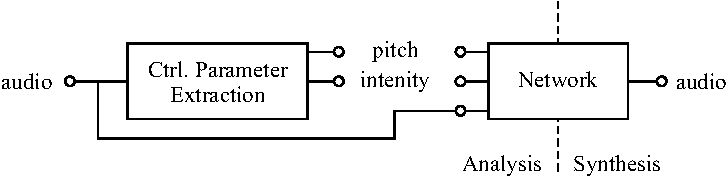
\includegraphics{Graphics/007_method_audio_predictor.pdf}
    \caption{Exemplary architecture of analysis and synthesis of audio predictor  singing voice synthesis methods.}
    \label{fig:method_audio_predictor}
\end{figure}

Audio predictor methods use deep neural networks to predict audio samples based on past predicted audio samples and conditioning signals such as pitch and intensity \cite{oord_wavenet:_2016}. One possible architecture is shown in figure \ref{method_audio_predictor}. During analysis, pitch and intensity trajectories have to be extracted from the source samples. The network is trained to predict new samples in the source audio by observing past samples and the conditioning signals. During synthesis, the network is used to predict new samples based on previously predicted samples (autorregression) and controlled via conditioning signals. A multi singer model can be trained by using multiple singer source samples together with a singer ID one-hot vector as conditioning signal during training. \\
End-to-End audio predictors are usually very complex due to the complexity of the task that the networks are responsible of \cite{engel_ddsp:_2020}.

\subsubsection*{Vocoder Predictor Methods}

\begin{figure}[H]
    \centering
    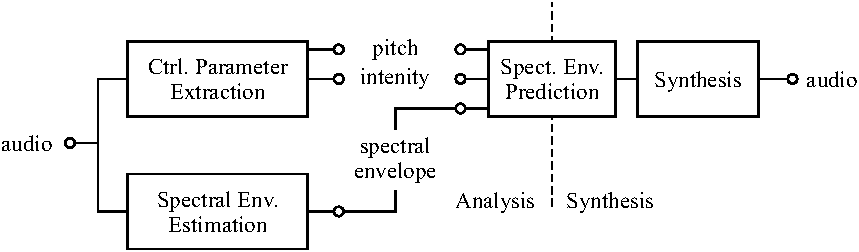
\includegraphics{Graphics/008_method_vocoder_predictor.pdf}
    \caption{Exemplary architecture of analysis and synthesis of vocoder predictor singing voice synthesis methods. }
    \label{fig:method_vocoder}
\end{figure}

Vocoder predictor methods are based on the source-filter model. One possible architecture is shown in figure \ref{method_vocoder}. Instead or predicting raw audio, they predict coefficients for a spectral envelope that can be used together with pitch and additional parameters to synthesize the audio. In  \cite{blaauw_neural_2017-1}, WaveNet was used to the predict the envelope coefficients autorregressively. Various vocoders can be used to extract spectral envelopes and synthesis audio \cite{morise_world:_2016}. One possible advantage over audio predictors is the reduced complexity of predicting spectral envelope parameters \cite{engel_ddsp:_2020}. Having access to spectral envelopes prior to synthesis also allows us to morph between singer models by interpolating between spectral envelopes prior to synthesis, for instance using their LSF representation \cite{roddy_method_2014}. 

\subsection*{Extended Source-Filter}
    
\begin{figure}[H]
    \centering
    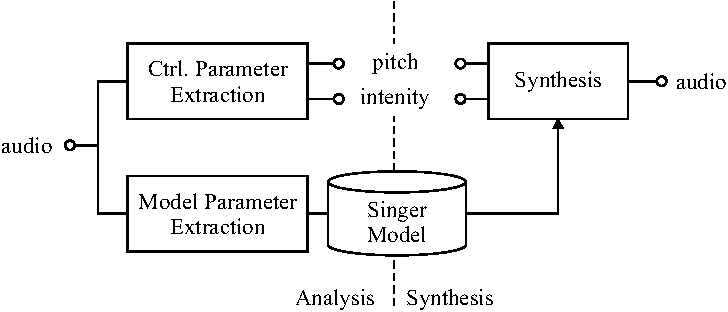
\includegraphics{Graphics/009_method_extended_source_filter.pdf}
    \caption{Exemplary architecture of analysis and synthesis of an extended source filter model for singing voice synthesis methods. }
    \label{fig:method_esf}
\end{figure}

Extended source-filter models require a high level of domain knowledge. The model would not only need to model vocal tract and glottal flow but also would need to model the dependency between control parameters pitch and intensity and the synthesis parameters for vocal tract and spectral envelope. During analysis, all parameters need to be estimated from the source sample. During synthesis, most parts of the model could be implemented using classical signal processing. This dramatically reduces the computational cost compared to the previously presented methods.\\
With vocal tract and glottal flow separated, morphing can be accomplished by interpolating their parameters respectively, again using representations such as LSF to achieve good results.

\subsubsection*{Differentiable DSP}

DDSP \cite{engel_ddsp:_2020} seems very promising but can't be easily applied to this thesis problem. As mentioned earlier, DDSP combines machine learning with classical DSP but requires the used DSP components to be differentiable. The commonly used model of the vocal tract as an all pole system however is not differentiable. With this limitation, no clean vocal tract separation could be achieved and DDSP could instead only be used to predict coefficients for a sinusoidal plus noise model \cite{serra_musical_1997}.

\subsubsection*{Summary - Singing Voice Synthesis Methods}

All three presented methods are suitable for implementing singing voice synthesis. However, with the computational complexity of audio prediction and vocoder prediction, an extended source-filter model is the currently preferred method considering the requirements mentioned earlier.\\

\subsection{Evaluation}

Evaluation of the proposed method is supposed to answer the following questions. Is the proposed method capable of recreating sung vowel excerpts to a satisfactory level? Can the method be used to synthesize sung vowel excerpts perceived as realistic or natural by listeners? Does the proposed model fulfil the strict real time requirements imposed on it? To answer the first two questions, an empirical user test is proposed. Since no hardware is necessary for this test, we suggest conducting an online survey to increase the potential number of participants. 

For measuring the perceived difference between original and synthesized excerpts, a MUSHRA (MUltiple Stimuli with Hidden Reference and Anchor) \cite{itu-r_recommendation_bs.1534_method_2003} test is proposed \cite{morise_cheaptrick_2015}\cite{morise_world:_2016}\cite{blaauw_neural_2017-1}. Alternatively, for small audibly differences, ABC-HR (ABC-Hidden Reference) \cite{itu-r_recommendation_bs.1534_method_2003} can be used instead. The synthesized excerpt is generated using the control parameter trajectories extracted from the original excerpt so that  the synthesized excerpt ideally is perceptually identical to the original excerpt. 

Additionally, some aspects of the method can be evaluated by performing a subjective paired comparison test as proposed in \cite{oord_wavenet:_2016}. In this test, the participants are asked to listen to two samples and state which they prefer with the option to choose "neutral". In all tests, sample $A$ is synthesized directly from model $A$ using the control parameters extracted from the original source audio sample $A$. If the method performs well, we expect a neutral response regarding which sample the participants prefer.

\begin{itemize}
    \item \textbf{Separation of voice timbre qualities and expressive qualities.}\\
    Sample $A$ is compared with an audio sample generated by using the same model $A$ but control parameters extracted from original sample $B$. This test measures how well a model transitions from it's original set of control parameters to a new set of control parameters.  
    \item \textbf{Voice Morphing Capabilities}\\
    The synthesized sample $A$ is compared with the synthesized sample $A \times B$, created by morphing models $A$ and $B$, using the same control parameters as with sample $A$. This test measures how well a morph between models maintains the naturalness of the voice.
\end{itemize}

\section{Preparatory Work}

This section describes work conducted in preparation for this master thesis. The biggest portion of which went into researching previous singing voice synthesis methods. Some effort was put into acquiring a better understanding of the human speech production system. A good understanding of the speech production system is important for this thesis mainly for defining a synthesis model that closely mimics the speech production system. Some time was spend studying modern approaches for source filter separation, filter envelope estimation and glottal flow models. The separation of the vocal tract filtering and the vocal folds oscillation (source) is a reoccurring challenge in singing voice synthesis. Finally, some time was devoted to researching machine learning approaches to singing voice synthesis.

In preparation for this thesis, some of the methods proposed in previous papers, including filter envelope estimators (LPC, TE) and glottal flow models (LF, LF-Rd) have been implemented in Matalb in order to get familiar with their performance, strengths and weaknesses. A framework for extract pitch, overtone frequencies and phases of sung vowel excerpts have been implemented using the programming environment Matlab. It was used to explore the VocalSet dataset\cite{wilkins_vocalset:_2018} and to analyse the included singing voice experts regarding spectral content and temporal fluctuation of pitch and overtone amplitude and phase. 

\section{Work and Timetable}

This section outlines the timetable for the thesis. The preparatory work prior to the thesis application included researching state of the art singing voice synthesis methods and defining the research questions. The main phase of the thesis consists of implementation, evaluation and thesis writing. The singing voice synthesis method is realized in an iterative manner with the implementation going hand in hand with additional research and intermediate evaluation phases. The final evaluation phase consists of an empirical test and is intended to validate the synthesis method on a perceptual level. Writing is supposed to last one month. Two months are reserved as optional time in case any of the other phases take longer then expected. A time schedule is provided in table \ref{table:time_schedule};

\begin{table}[H]
  \centering
    \renewcommand{\arraystretch}{1.5}
  \begin{tabular}{c | c ? c | c |c | c ? c | c}
  \hline
    January & February & March & April & May & June & July & August \\\hline 
    \multicolumn{2}{c?}{Preparatory} & \multicolumn{4}{c?}{Thesis} & \multicolumn{2}{c}{Buffer}\\\hline
    Research & Proposal & \multicolumn{2}{c|}{Implementation} & \multicolumn{1}{c|}{Evaluation} & \multicolumn{1}{c?}{Writing} & \multicolumn{2}{c}{}\\\hline 
  \end{tabular}
  \label{table:time_schedule}
  \caption{The proposed work time plan for the master thesis.}
\end{table}

\subsection{Agenda}

This section roughly outlines the remaining tasks that comprise this thesis.

\subsubsection*{Preparatory Work}
\begin{itemize}
    \item Compile and Summarize prior research in the field of singing voice synthesis.
    \item Write the exposé for the thesis application.
\end{itemize}

\subsubsection*{Implementation}
\begin{itemize}
    \item Define a method following the requirements laid out in this document.
    \item Iterative prototyping of the proposed method, conducting additional research and evaluation phases when necessary. 
    \item Source code refactoring and documentation.
\end{itemize}


\subsubsection*{Evaluation}
\begin{itemize}
    \item Compile material (synthesized and original audio excerpts) for the empirical test
    \item Design an empirical test / online survey
    \item Implement the online survey using tools such as LimeSurvey
    \item Run and maintain the survey
    \item Collect and analyse test results 
\end{itemize}

\subsubsection*{Writing}
\begin{itemize}
    \item Write the master thesis 
    \item Write German summary of the thesis
    \item Iterative proofreading and improving of content and writing
    \item Final proofreading and spellchecking
\end{itemize}

\newpage
%\bibliography{zotero_references.bib}
\printbibliography

\end{document}


